\section{Thiết kế hệ thống}
\subsection{Hệ thống xử lý câu truy vấn SQL}
\hspace*{1cm} Để có thể xử lý câu truy vấn được nhập từ User. Nghiên cứu các giải pháp sao cho có thể nhận câu SQL người chơi đã nhập, xử lý và trả kết quả về cho hệ thống xử lý và đưa ra các phản ứng của game. Có rất nhiều hướng tiếp cập khác nhau. Nhưng nhóm cũng lựa chọn một số hướng tiếp cận nhất định.
\subsubsection{Hướng tiếp cận sử dụng SQL Server tại Localhost}
\hspace*{1cm} Hướng tiếp cận này sử dụng module SQL và DB là một process độc lập và việc giao tiếp giữa DB và Game là thông qua việc kết nối Database thông qua địa chỉ Localhost và một port nhất định. Việc thiết lập SQL Database Server là riêng biệt. Về phía Game Client chỉ gần thiết lập một connector, sử dụng làm client rồi kết nối đến process Server Local. Các câu truy vấn và dữ liệu trả về sẽ được giao tiếp thông qua connector này.
\begin{figure}[H]
	\centering
	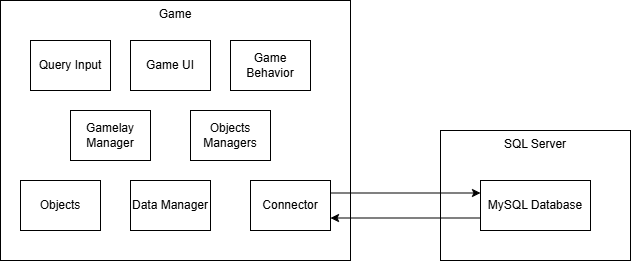
\includegraphics[width=\textwidth]{Images/SQLLocalServer.png}
	\vspace{0.5cm}
	\caption{Mô hình cấu trúc của hướng giải pháp chạy SQL Server trên Local}
\end{figure}
Dưới đây là đoạn code mẫu cho việc kết nối đến SQL Server và gọi yêu cầu thực thi truy vấn từ client\\
\begin{verbatim}
	using System;
	using MySql.Data.MySqlClient;
	
	public class DatabaseConnection
	{
		private MySqlConnection connection;
		
		public void Initialize()
		{
			string connectionString = "Server=localhost;Database=yourdatabase;Uid=yourusername;Pwd=yourpassword;";
			connection = new MySqlConnection(connectionString);
		}
		
		public void OpenConnection()
		{
			try
			{
				connection.Open();
				Console.WriteLine("Connection opened successfully.");
			}
			catch (Exception ex)
			{
				Console.WriteLine("An error occurred: " + ex.Message);
			}
		}
		
		public void CloseConnection()
		{
			try
			{
				connection.Close();
				Console.WriteLine("Connection closed successfully.");
			}
			catch (Exception ex)
			{
				Console.WriteLine("An error occurred: " + ex.Message);
			}
		}
		
		public void ExecuteQuery(string query)
		{
			try
			{
				OpenConnection();
				MySqlCommand cmd = new MySqlCommand(query, connection);
				cmd.ExecuteNonQuery();
				Console.WriteLine("Query executed successfully.");
			}
			catch (Exception ex)
			{
				Console.WriteLine("An error occurred: " + ex.Message);
			}
			finally
			{
				CloseConnection();
			}
		}
	}
\end{verbatim}
\hspace*{1cm} Với việc sử dụng một process riêng, ta có thể tuỳ biến process theo dạng Hệ cơ sở dữ liệu SQL nào đều được, bao gồm MySQL, PostgreSQL,... Miễn là ta lựa chọn thư viện Database Client cho Connector phù hợp là được. Ta sẽ có toàn bộ chức năng như một hệ cơ sở dữ liệu thuần tuý, ta có thể thiết lập các stored procedure, function, thiết lập các quyền cho các user khác nhau cũng như nhiều tính năng hỗ trợ hơn.\\
\hspace*{1cm} Tuy nhiên, với việc sử dụng một process riêng và có sử dụng port. Nếu không xử lý port hợp lý, port mà process chiếm dụng sẽ không được sử dụng cho mục đích khác nữa. Hơn nữa, việc chạy localhost server bản chất vẫn là process, và nó có thể chấm dứt bởi trình quản lý tác vụ của hệ điều hành. Nếu mất đi kết nối với server local, game sẽ không thể thực thi các tác vụ có liên quan đến SQL, game sẽ không thể hoạt động và đó là điều không thể chấp nhận được. Hơn nữa, việc khởi chạy game đòi hỏi game cũng phải khởi chạy thêm tiến trình server. Cũng như khi cài đặt trò chơi, ta phải cài đặt thêm SQL Server. Khiến cho cấu trúc lủng củng, không nhất quán, đặc biệt là nếu SQL Server có sự cố thì game cũng không hoạt động được, dẫn đến chạy không ổn định.
\subsubsection{Hướng tiếp cận xây dựng Hệ cơ sở dữ liệu SQLite ngay trong game}
\hspace*{1cm} Thay vì sử dụng một process riêng biệt, hướng tiếp cận này sử dụng SQLite, là một hệ cơ sở dữ liệu gọn nhẹ, có khả năng nhúng vào các ứng dụng khác. Đây là một ưu điểm lớn của SQLite khi nó có thể thực hiện các câu truy vấn ngay trong lòng ứng dụng, giúp cho cấu trúc được nhất quán và hoạt động đồng nhất và ổn định.
\begin{figure}[H]
	\centering
	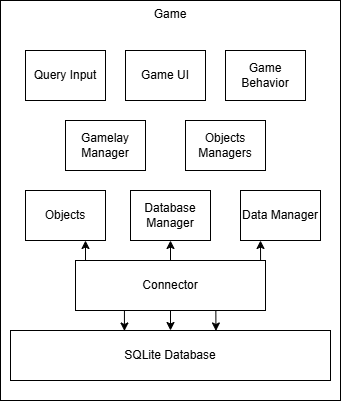
\includegraphics[width=\textwidth]{Images/SQLITE.png}
	\vspace{0.5cm}
	\caption{Cấu trúc game với Hệ cơ sở dữ liệu SQLite}
\end{figure}